%\section{Tensor Factorization}  \label{sec:tf}

\section{Multiverse Factorization Model} \label{sec:tf}
Factorization models for tensors are studied for many years~\cite{karatzoglou2010multiverse}. The main idea behind the use of  Tensor Factorization (TF) is that we can take advantages of the principle behind Matrix Factorization to deal with multi-Order information. In sensor network, Temporal informations, spatial informations and  heterogeneous sensors informations are strongly correlated. Modeling the correlation between them will be a great benefit to recovery the missing value.
 
Tensor decomposition is a multi-dimensional extension of Singular Value Decomposition. In the section 4.1 we introduce the methods of Tensor Decomposition. A general model of tensor decomposition is the Tucker decomposition (TD) also known as High-Order Singular Value Decomposition (HOSVD). The special case of Tucker decomposition is called canonical decomposition (CD) also known as the parallel factor analysis (PARAFAC).
However, the Tensor Decomposition methods require a dense input matrix R and therefore ignore the missing part of  input data. Treating R as a dense tensor with missing entries being assume to be 0. It would make predict missing value failed. We introduce and explain the details of how we have adapted the Tensor Decomposition models with latent features for missing value recovery in section 4.2.  

\subsection{Tensor Decomposition}

 If we want to decompose a $m\times n$ Matrix M, recall the Singular Value Decomposition(SVD) as being
\begin{equation*} 
\mathbf{M}=\mathbf{P}\Sigma \mathbf{Q}^\mathrm{T}=\sum\limits_{k=1}^r\sigma_kp_kq_k^\mathrm{T}=\sum\limits_{k=1}^r\sigma_kp_k\otimes q_k
\end{equation*}
Where $\otimes$ denoted the tensor product : $x\otimes y = xy^\mathrm{T}$. $r$ is the rank of M,
P is an $m\times m$ unitary matrix, Q is a $n\times n$ unitary matrix, $\Sigma$ is an $m\times n$ rectangular diagonal matrix with singular values of M, being adopted the following convention $\sigma_1>\sigma_2 >...\sigma_r>0=\sigma_{r+1}=...=\sigma_{n}$. The SVD may be generalized to High-Order Tensor decomposition. the following are two types of tensor decomposition, for simplicity and in practical, we present the decomposition for tensor of order q=3.

\subsubsection{Tucker Decomposition}
The Tucker decomposition
was �rst introduced by Tucker in 1963 [1], it factorizes a higher-order tensor into a core tensor S and a factor matrix for each dimensions. we decompose a $m\times n \times c $ tensor T :

\begin{equation*}
\mathbf{T}=\sum\limits_{i=1}^{r_1}\sum\limits_{j=1}^{r_2}\sum\limits_{k=1}^{r_3}\mathbf{S}_{ijk}p_i\otimes q_j\otimes w_k
\end{equation*}
or for each components,
\begin{equation*}
\mathbf{T}_{\alpha\beta\gamma}=\sum\limits_{i=1}^{r_1}\sum\limits_{j=1}^{r_2}\sum\limits_{k=1}^{r_3}\mathbf{S}_{ijk}P_{\alpha i}Q_{\beta j}W_{\gamma k}
\end{equation*}
Where the vector $p_i$, $q_j$, and $w_k$ are the column of matrices P, Q and W respectively, which are the factor matrices (usually orthogonal). They can be thought of as the principal components in each order There are several algorithms for calculating Tucker decompositions. For data compression, the Tucker decomposition usually assume that $r_1\le m$, $r_2 \le n $ and $r_3 \le c$. 
\subsubsection{Canonical Decomposition}

The Canonical  decomposition factorizes a tensor into a sum of component rank-one
tensors. Formally, the Canonical Decomposition(CD) is the special case of the Tucker decomposition
when S is superdiagonal. The Canonical Decomposition of T is
\begin{equation*}
\mathbf{T}=\sum\limits_{i=1}^{k}x_i\otimes y_i\otimes z_i
\end{equation*}
or
\begin{equation*}
\mathbf{T}_{\alpha\beta\gamma}=\sum\limits_{i=1}^{k}X_{\alpha i} Y_{\beta i} Z_{\gamma i}
\end{equation*}

Here the $x_i$,$y_i$ and $z_i$ are the column of matrices X, Y and Z, which are the factor matrices, k is the factor size. 

The Tucker Decomposition and Canonical Decomposition are illustrated in Figure 1.


\begin{figure}[h] 
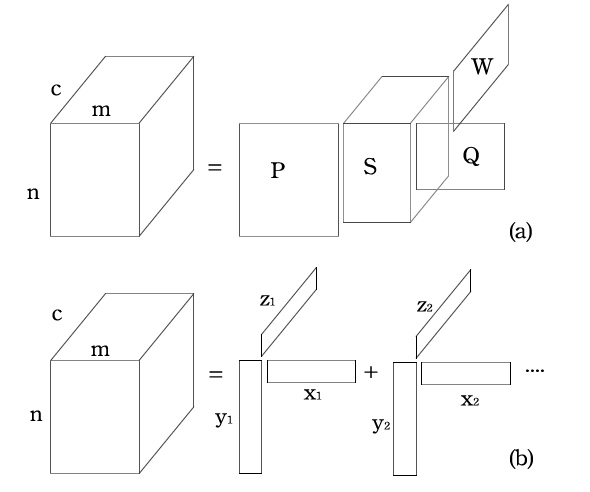
\includegraphics[width=9cm]{tf.jpg} 
\caption{ (a) the Tucker Decomposition model  (b) the Canonical Decomposition model is a special case of TD model. In sensor network, the three dimension can be nominal features such as node id, time frame number.
}


\end{figure}



\subsection{Tensor Factorization for missing recovery}
\subsubsection{Objective function}

Existing Tensor Decomposition model is requiring the dense tensor, which is unsuitable for missing data recovery when the missing rate increased. Therefore, we propose an N-order Tensor Factorization  for missing data recovery. Just like MF, it take advantage of sparsity of the data while still exploiting the temporal correlation. Moreover, it models the correlation between different informations, e.g. spatial correlation, heterogeneous sensor readings. The followings are the details of the model we proposed.

Assume that there are three features $F_1, F_2 , F_3$, $F_1$ is the time frame number, $F_2$ and $F_3$ are the other features, it could be the sensor node ID, sensor node coordinates, heterogeneous sensor readings or other information. suppose the target sensor readings is $R$ such that tensor T containing  $R$ will be 3-dimensional tensor :
\begin{equation*}
T := F_1 \times  F_2 \times F_3 \rightarrow R
\end{equation*}

In contrast to tensor decomposition, the learning model we propose is learning the latent factors P, Q, W. Where P, Q, W are the factors of $F_1, F_2, F_3$. To avoid over-fitting and decrease the complexity of computing prediction, our model is based on Canonical Decomposition. Its complexity of computing prediction is $O(k)$, where k is the factor size of  P, Q and W. On the other hand, the complexity of Tuker Decomposition is $O(k^3)$  by our optimization method,
where $ k=min(k_P,k_Q,k_W) $ , $k_P$, $k_Q$, $ k_W$ are the factor size of P, Q, W respectively.


As MF, to increase the prediction accuracy, we also add bias term of $F_1, F_2, F_3$ into our Tensor Factorization model.
so our prediction function is :
\begin{equation*}
\begin{aligned}
\mathbf{\hat{T}}_{\alpha\beta\gamma}=\mu_\alpha+\mu_\beta+\mu_\gamma+p_\alpha q_\beta w_\gamma
\\=\mu_\alpha+\mu_\beta+\mu_\gamma+\sum\limits_{i=1}^{k}P_{\alpha i} Q_{\beta i} W_{\gamma i}
\end{aligned}
\end{equation*}
to learn the latent features P, Q and W, we define the loss function :
\begin{equation*}
L(\mathbf{\hat{T}},\mathbf{T})=\frac{1}{\|D\|_1} \sum\limits_{t\in D}  l(\hat{t},t)
\end{equation*}
where $D$ is the dataset and $\|D\|$ means the amounts of data point. $l$ is a point-wise loss function penalizing the distance between estimate and observation. we choose $l$ being least squared error because the evaluation function is root mean square error (RMSE), so
\begin{equation*}
l(\hat{t},t)=\frac{1}{2}(t-\hat{t})^2
\end{equation*}

Simply minimizing a loss function is known to lead to over-fitting. Given the factors P, Q, W and bias terms which constitute our model, we have a choice of ways to ensure that the model complexity does not grow without bound. we add a regularization term based on the $l_2$ norm of these
factors. To capture the temporal effect, similar to MF we state previous in section 3.2, we add the time regularization term to our model.
Finally, the objective function of tensor factorization is :\\
\begin{equation*}
\begin{aligned}
&\sum\limits_{\alpha, \beta, \gamma} l( \hat{T}_{\alpha\beta\gamma}, T_{\alpha\beta \gamma} )+\lambda_1\|p_{\alpha}\|^2+\lambda_2\|q_\beta\|^2+\lambda_3\|w_\gamma\|^2+\lambda_4\|
\mu_\alpha\|^2\\
&+\lambda_5\|\mu_\beta\|^2+\lambda_6\|\mu_\gamma\|^2+\frac{1}{2}\lambda_7\sum(\mu_\alpha-\mu_{\alpha+1})^2+(\mu_\alpha-\mu_{\alpha-1})^2
\\&
+\frac{1}{2}\lambda_8\sum(p_\alpha-p_{\alpha+1})^2+(p_\alpha-p_{\alpha-1})^2
\end{aligned}
\end{equation*}

\begin{algorithm}[h]
  \caption{Multiverse Tensor Factorization}
  \label{alg::conjugateGradient}
  \begin{algorithmic}[1]
    \Require
    $\lambda_1,\lambda_2, \lambda_3, \lambda_4, \lambda_5, \lambda_6, \lambda_7, \lambda_8, \eta, k$
    \State Normalize the training set as $D$
    \State initial the $p_\alpha, q_\beta, w_\gamma, \mu_\alpha, \mu_\beta, \mu_\gamma$ for all $\alpha, \beta, \gamma$
    \Repeat
      \For    {each observed readings t in D}
      \State Update $p_\alpha, q_\beta, w_\gamma, \mu_\alpha, \mu_\beta, \mu_\gamma$ 
     \EndFor
     \State Update $p_\alpha,  \mu_\alpha $ for all u
    \Until stopping criterion is met
    \State Output the model 
  \end{algorithmic}
\end{algorithm}

\subsubsection{Optimization}
Minimizing this objective function can be done using many approaches. To deal with large datasets, there are simple and fast online algorithm which performs stochastic gradient descent (SGD) in the factors for a given tuple t simultaneously. we need to compute the gradients of the objective function with respect individual components of the model. Focus on a observed data t = $T_{\alpha\beta\gamma } $ from training data, the update rule is :
\begin{equation*}
\begin{aligned}
&{p_\alpha}^\prime={p_\alpha}+\eta(e*q_\beta w_\gamma - \lambda_1 p_\alpha)
\\&{q_\beta}^\prime={q_\beta}+\eta(e*p_\alpha w_\gamma - \lambda_2 q_\beta)
\\&{w_\gamma}^\prime={w_\gamma}+\eta(e*p_\alpha q_\beta - \lambda_3 w_\gamma)
\\&{\mu_\alpha}^\prime=\mu_\alpha+\eta(e-\lambda_4\mu_\alpha)
\\&{\mu_\beta}^\prime=\mu_\beta+\eta(e-\lambda_5\mu_\beta)
\\&{\mu_\gamma}^\prime=\mu_\gamma+\eta(e-\lambda_6\mu_\gamma)
\end{aligned}
\end{equation*}
where $e=t-\hat{t}$, After a iteration, we update the model according to the temporal regularization :
\begin{equation*}
\begin{aligned}
&{p_\alpha}^\prime={p_\alpha}+\eta\lambda_7(p_{\alpha+1}-p_\alpha+p_{\alpha-1}-p_\alpha)
\\&{\mu_\alpha}^\prime=\mu_\alpha+\eta\lambda_8(\mu_{\alpha+1}-\mu_\alpha+\mu_{\alpha-1}-\mu_\alpha)
\end{aligned}
\end{equation*}
The Tensor Factorization method is summarized in Procedure 2, which is easy to implement since it accesses only one row of P, Q ,W at a time. 
The details about normalization, initialization and stop criterion are just like MF, which are stated in previous part. The parameters of TF are more than MF, but we can achieve reasonable performance by setting
\begin{equation*}
\begin{aligned}
& \lambda_1=\lambda_2=\lambda_3,\\
& \lambda_4=\lambda_5=\lambda_6\\
&\lambda_7=\lambda_8\\
\end{aligned}
\end{equation*}
